\documentclass{article}
\usepackage{graphicx} % Required for inserting images
\usepackage{yehyun}

\title{Notes on General Relativity}
\author{Yehyun Choi}

\begin{document}

\maketitle

\pagebreak

\section{Preliminaries}
\textcolor{red}{Wald Ch. 2, Carroll Ch. 2-3}

An $n$-dimensional $C^\infty$ real \textbf{manifold} $M$ is defined as a set with a collection of subsets $\{O_a\}$ that satisfy:
\begin{enumerate}
    \item Each $p\in M$ lies in at least one $O_a$; the $\{O_a\}$ cover $M$.
    \item For each $\alpha$, there is a bijective map $\psi_a:O_a\to U_a$, where $U_a$ is open in $\mathbb R^n$.
    \item If $O_a\cap O_\beta\ne\emptyset$, then $\psi_\beta\circ\psi_\alpha^{-1}$ is $C^\infty$.
\end{enumerate}
Some examples include $\mathbb R^3$, $\mathbb R^d$, $S^2$, and $T^2$. Anti-examples include cones and discrete manifolds.


In $\mathbb R^n$, a vector $v=(v^1,\cdots,v^n)$ defines the directional derivatives and vice versa. For a manifold, \textbf{Tangent vectors} are maps $v:\mathcal F\to\mathbb R$ characterized by linearity and Leibnitz rule; for $\mathcal F$, a field of $C^\infty:M\to\mathbb R$, 
\begin{enumerate}
    \item $v(af+bg)=av(f)+bv(g),\,\forall f,g\in\mathcal F;\,a,b\in\mathbb R$.
    \item $v(fg)=f(p)v(g)+g(p)v(f).$
\end{enumerate}

\begin{figure}[h]
    \centering
    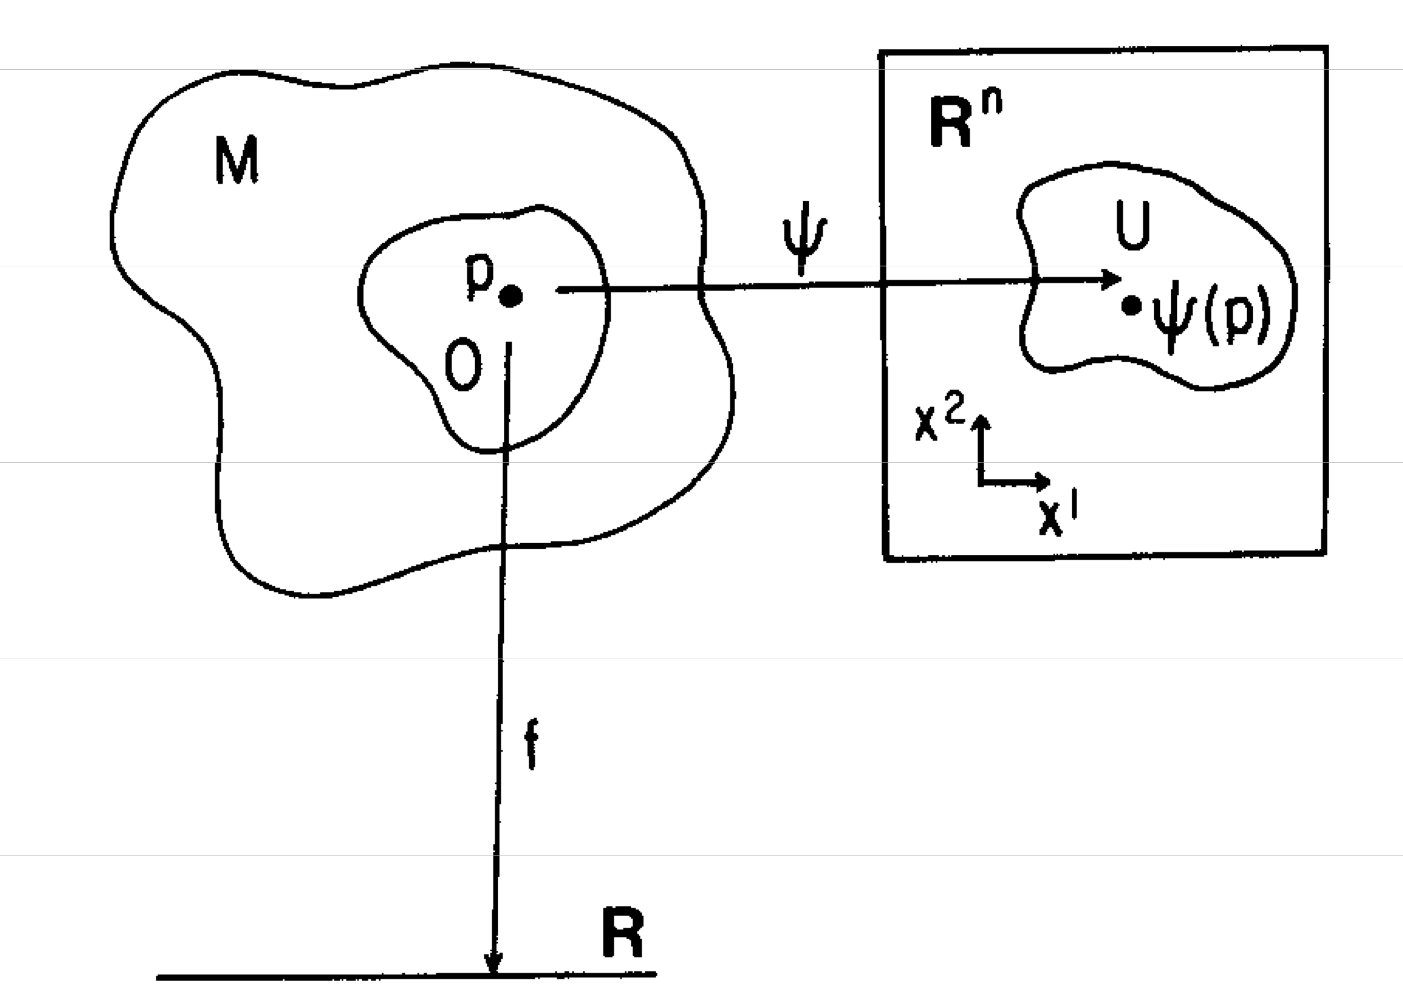
\includegraphics[width=0.5\linewidth]{images/gr-images/5339.jpg}
    \caption{A diagram illustrating the definition of the directional derivatives $X_\mu$}.
    \label{fig:enter-label}
\end{figure}

Now, we construct the basis of $V_p=\{v\}$. We define $X_\mu:\mathcal F\to\mathbb R$ by 
$$X_\mu(f)=\left.\pde{}{x^\mu}(f\circ\psi^{-1})\right|_{\psi(p)}.$$
Using Haadmard's lemma (\textcolor{red}{Wald thm. 2.2.1})
$$v=\sum^n_{\mu=1}v^\mu X_\mu,\quad v^\mu=v(x^\mu\circ\psi).$$
Typically, we denote $X_\mu$ as $\pde{}{x^\mu}$. 

Using the chain rule, we can show the vector transformation law:
$$X_\mu=\left.\sum^n_{\nu=1}\pde{x'^\nu}{x^\mu}\right|_{\psi(p)}X'_\nu,\quad v'^\nu=\sum^n_{\mu=1}v^\mu\pde{x'^\nu}{x^\mu}.$$
Let $C:\mathbb R\to M$ be a $C^\infty$ map - think worldlines. At point $p\in M$, $C$ is related to a tangent vector $T$ as $T(f)=\ode{f\circ C}t$:
$$T(f)=\ode{}{t}(f\circ C)=\sum_\mu\pde{}{x^\mu}(f\circ\psi^{-1})\ode{x^\mu}t=\sum_\mu\ode{x^\mu}tX_\mu(f)\implies T^\mu=\ode{x^\mu}t.$$

Let $V$ be a finite dimensional vector space. Consider the vector space $V^*$ of linear maps $f:V\to\mathbb R$. For $v_1,\cdots,v_n$ basis of $V$, define $v^{1*},\cdots,v^{n*}\in V^*$ by 
$$v^{\mu*}(v_\nu)=\delta^\mu_\nu.$$
Now, we define a tensor $T$ of type $(k,l)$ over $V$ as 
$$T:V^*\times\cdots\times V^*\times V\times\cdots\times V\to\mathbb R.$$
Obviously, the vector space $\mathbb T(k,l)$ is $n^{k+l}$. 

Let $\{v_\mu\}$ be a basis of $V$ and $\{v^{\nu*}\}$ its dual basis; from multilinearity, a basis of $\mathbb T(k,l)$ can be $\{v_{\mu_1}\otimes\cdots\otimes v_{\mu_k}\otimes v^{\nu_1*}\otimes\cdots\otimes v^{\nu_l*}\}$:
$$T=\sum^n_{\mu_1,\cdots,\nu_l=1}T\indices{^{\mu_1\cdots\mu_k}_{\nu_1\cdots\nu_1}}v_{\mu_1}\otimes\cdots\otimes v^{\nu_l*}.$$

We now define two operators on tensors. The first operation is the \textbf{contraction}; defined with the $i$th and $j$th slots is the map $C:\mathbb T(k,l)\to\mathbb T(k-1,l-1)$, defined
$$CT=\sum^n_{\sigma=1}T(\cdots,v^{\sigma*},\cdots;\cdots,v_\sigma,\cdots),$$
where $\{v_\sigma\}$ is a basis of $V$, $\{v^{\sigma*} \}$ is its dual basis.

The second operation is the \textbf{outer product}. Given a tensor $T(k,l)$ and another tensor $T'(k',l')$, we construct tensor $T\otimes T'(k+k',l+l')$. It is simply defined
$$T\otimes T'=T(v^{1*},\cdots,v^{k*};w_1,\cdots,w_l)T'(v^{k+1*},\cdots,v^{k+k'*};w_{l+1},\cdots,w_{l+l'}).$$

In the case that $V_p$ is the tangent space to manifold $M$ at point $p$, $V^*_p$ is the cotangent space. If the coordinate basis of $V_p$ is $\left\{\pde{}{x^1},\cdots,\pde{}{x^n}\right\}$, the associated dual basis is $\dd x^1,\cdots,\dd x^n$. It is defined that $\dd x^\mu\left(\pde{}{x^\nu}\right)=\delta^\mu_\nu.$

It follows that the dual vector $\omega$, in the dual basis $\{\dd x^\mu\}$, transforms 
$$\omega'_{\mu'}=\sum^n_{\mu=1}\omega_\mu\pde{x^\mu}{x'^\mu}.$$
Likewise,
$${T'}\indices{^{\mu'_1\cdots\mu'_k}_{\nu'_1\cdots\nu'_l}}=\sum^n_{\mu_1,\cdots,\nu_l=1}T\indices{^{\mu_1\cdots\mu_k}_{\nu_1\cdots\nu_l}}\pde{{x'}^{\mu'_1}}{x^{\mu_1}}\cdots\pde{x^{\nu_l}}{{x'}^{\nu'_l}}.$$
As an example, the metric is a rank $(0,2)$ tensor. 


In a metric space, the metric is defined; one can think of it as the ``infinitesimal square distance'' or as something that defines the inner product in the tangent space (which, in turn, is the natural isomorphism between the tangent space and the cotangent space)
$$g=\sum_{\mu,\nu}g_{\mu\nu}\dd x^\mu\otimes\dd x^\nu,\quad\dd s^2=\sum_{\mu,\nu}g_{\mu\nu}\dd x^\mu\dd x^\nu.$$

We can always find a coordinate system such that $g_{\mu\nu}(p)=\eta_{\mu\nu}$ and $\partial_\sigma g_{\mu\nu}(p)=0$, making the metric locally inertial.

A tensor is said to be symmetric if it's unchanged under exchange of its indices; $S_{\mu\nu\rho}=S_{\nu\mu\rho}$. It's antisymmetric (about given indices) if it changes sign when those indices are exchanged: $A_{\mu\nu\rho}=-A_{\rho\nu\mu}$. One can symmetrize/antisymmetrize tensors by taking the sums:


It is useful to define the \textbf{levi-civita symbol} as a tensor. It is defined (note that here, $\tilde\epsilon$ is the symbol):

$$\epsilon_{\mu_1\mu_2\cdots\mu_n} = \sqrt{|g|} \tilde{\epsilon}_{\mu_1\mu_2\cdots\mu_n}, \quad \epsilon^{\mu_1\mu_2\cdots\mu_n} = \frac{1}{\sqrt{|g|}} \tilde{\epsilon}^{\mu_1 \mu_2 \cdots \mu_n}.$$
For $p$ and $q$ forms, the \textbf{wedge product}, $\wedge:\omega_p,\omega_q\to\omega_{p+q}$ is defined 
$$(A\wedge B)_{\mu_1\cdots\mu_{p+q}}=\frac{(p+q)!}{p!q!}A_{[\mu\cdots\mu_p}B_{\mu_{p+1}\cdots\mu_{p+q}]}.$$
The \textbf{exterior derivative} $d:\omega_p\to\omega_{p+1}$ is defined 
$$(dA)_{\mu_1\cdots\mu_{p+1}}=(p+1)\partial_{[\mu_1}A_{\mu_2\cdots\mu_{p+1}]}.$$
The \textbf{Hodge symbol} $*:\omega_p\to\omega_{n-p}$, where $n$ is the dimensionality of the maniofld, is defined 
$$(*A)_{\mu_1\cdots\mu_{n-p}}=\frac 1{p!}\epsilon\indices{^{\nu_1\cdots\nu_p}_{\mu_1\cdots\mu_{n-p}}}A_{\nu_1\cdots\nu_p}\implies **A=(-1)^{s+p(n-p)}A,$$
where $s$ is the number of minus signs in the eigenvalues of the metric.

We define the \textbf{covariant derivative} as a covariant map $\nabla:T^\mu_\nu\to T^\mu_{\nu+1}$, having properties:
\begin{enumerate}
    \item Linearity: $\nabla(T+S)=\nabla T+\nabla S$;
    \item Leibniz rule: $\nabla(T\otimes S)=(\nabla T)\otimes S+T\otimes(\nabla S)$;
    \item Commutes with contractions: $\nabla_\mu(T\indices{^\lambda_{\lambda\rho}})=(\nabla T)\indices{_\mu^\lambda_{\lambda\rho}}$;
    \item Reduces to partial on scalars: $\nabla_\mu\phi=\partial_\mu\phi$.
\end{enumerate}
A covariant derivative satisfying such properties takes the form 
$$\nabla_\mu V^\nu=\partial_\mu V^\nu+\Gamma^\nu_{\mu\lambda}V^\lambda,\quad \nabla_\mu\omega_\nu=\partial_\mu\omega_\nu-\Gamma^\lambda_{\mu\nu}\omega_\lambda.$$
In general relativity, we impose that the metric satisfies two more conditions:

\begin{enumerate}
  \setcounter{enumi}{4}
  \item Torsion free - connection symmetric in lower indices: $\Gamma^\lambda_{\mu\nu}=\Gamma^\lambda_{(\mu\nu)}$;
  \item Metric compatibility: $\nabla_\rho g_{\mu\nu}=0$.
\end{enumerate}

In this case, the connection coefficients are called the \textbf{Chrisftoffel symbols}:
$$\Gamma^\rho_{\mu\nu}=\frac 12g^{\sigma\rho}(\partial_\mu g_{\nu\rho}+\partial_\nu g_{\rho\mu}-\partial_\rho g_{\mu\nu}).$$

We define the parallel transport of the tensor $T$ along the path $x^\mu(\lambda)$ to be the requirement that the covariant derivative along the path vanishes:
$$\left(\frac{D}{d\lambda}T\right)\indices{^{\mu_1\mu_2\cdots\mu_k}_{\nu_1\nu_2\cdots\nu_l}}=\ode {x^\sigma}\lambda\nabla_\sigma T\indices{^{\mu_1\mu_2\cdots\mu_k}_{\nu_1\nu_2\cdots\nu_l}}=0\implies \ode{}{\lambda}V^\mu+\Gamma^\mu_{\sigma\rho}\ode{x^\sigma}\lambda V^\rho=0.$$
We define a geodesic to be a curve that parallel-transports its own tangent vector:
$$\frac{D}{d\lambda}\ode{x^\mu}\lambda=0\implies\oden 2{x^\mu}\lambda+\Gamma^\mu_{\rho\sigma}\ode{x^\rho}\lambda\ode{x^\sigma}\lambda=0.$$

Note that we have an affine parameter; the geodesic equation is invariant under a linear transformation $\lambda\to a\lambda+b.$ With this freedom, we choose
\begin{enumerate}
    \item for massive particles, $p^\mu=mu^\mu=m\ode{x^\mu}\tau$,
    \item for massive particles, $p^\mu=\ode{x^\mu}\lambda$, $p^2=0$.
\end{enumerate}

Let $k^\mu$ be a vector at point $p$. It defines a geodesic curve $x^\mu$. We define \textbf{Riemann normal coordinates} as $x^\mu(\lambda)=\lambda k^\mu$, which is locally inertial.

We define an isometry\footnote{In case of $\mathbb R^n$, there are $n$ translations and $\frac 12n(n+1)$ rotations, giving us $\frac n2(n+1)$ killing vectors. Manifolds with $\frac n2(n+1)$ isometries are called \textbf{maximally symmetric}. Other maximally symmetric manifolds include: $\mathbb R^n$, $S^n$, $\mathbb H^n$ spatially, and $\mathbb R^{n-1,1},$ $\dd S_n$, and Ad$S_n$. 
} as a map $f:M\to M$ with $d(f(p_1),f(p_2))=d(p_1,p_2)$. Infinitesimally, we can parametrize $f$ by a vector field $\zeta^\mu$: for $p\to f(p)$, we have $x^\mu\to x^\mu+\zeta^\mu(x)$ and hence $\delta x^\mu=\zeta^\mu(x)$. Isometry requires that $\delta(ds^2)=0$, giving us 
$$\delta(\dd s^2)=\delta(g_{\mu\nu}\dd x^\mu\dd x^\nu)=\partial_\alpha g_{\mu\nu}\delta x^\alpha\dd x^\mu\dd x^\nu+2g_{\mu\nu}\dd(\delta x^\mu)\dd x^\nu=(\delta_\zeta g_{\mu\nu})\dd x^\mu\dd x^\nu,$$
where we have defined 
$$\mathcal L_\zeta g_{\mu\nu}=\delta_\zeta g_{\mu\nu}=\zeta^\alpha\partial_\alpha g_{\mu\nu}+\partial_\mu\zeta^\alpha g_{\alpha\nu}+\partial_\nu\zeta^\alpha g_{\mu\alpha},$$
which is known as the \textbf{Lie derivative}. We can then rewrite the isometry statement in two ways:
$$\delta(\dd s^2)=0\implies\mathcal L_\zeta g_{\mu\nu}=0,\quad \nabla_{(\mu}\zeta_{\nu)}=0.$$
The second equation is called the \textbf{Killing equation}. The coordinates in which locally, $\zeta=\partial_x$ hae obvious symmetries - in these coordinates, the isometries, finite or infinitesimal, are trivial translations. 

Each Killing vector corresponds to a conserved quantity, $p_\zeta=p^\alpha\zeta_\alpha$ along geodesics; 
$$\ode{p_\zeta}\tau=p^\mu\partial_\mu(p^\alpha\zeta_\alpha)=p^\mu\nabla_\mu(p^\alpha\zeta_\alpha)=(p^\mu\nabla_\mu p^\alpha)\zeta_\alpha+p^\mu p^\alpha\nabla_\mu\zeta_\alpha.$$
The first term is zero from the geodesic equation and the second from the Killing equation. As an example, $E=-\zeta^\alpha p_\mu$ as a conserved quantity\footnote{Since the observed energy is $-u^\alpha p_\alpha$ where $u$ is the velocitiy of the observer; hence, $E_\text{obs}=E$ only if $\zeta$ is timelike.}.


\pagebreak
\section{Intro}

\textcolor{red}{Add section for SR? - Carroll ch.1, Hartle ch.4}

The \textbf{postulates of SR} state
\begin{enumerate}
    \item Spacetime is the geometry with the (Minkowski) metric $\dd s^2=-c^2\dd t^2+\dd x^2+\dd y^2+\dd z^2$; speed of light is the same in all frames. This was realized from electromagnetism.
    \item The laws of physics are tensor equations; physics is the same in all inertial frames.
\end{enumerate}

The symmetries in Minkowski spacetime are called Poincare transformations, defined $x'^\alpha=\Lambda^\alpha_\beta x^\beta+a^\alpha$, with 4 transformations in $a^\alpha$, and 3 rotations and 3 boosts in Lorentz transformations, defined $\eta=\Lambda^\intercal\eta\Lambda$. These form the Lorentz group, $O(3,1)$, consisting of combinations of proper/restricted Lorentz transformation, time reversal $T$, parity reversal $P$, and $PT$. 

Using the definition, we can find the generators of the Lorentz group: for an infinitesimal transformation $\Lambda^\alpha_\beta=\delta^\alpha_\beta+\omega^\alpha_\beta$, $\Lambda^\intercal\eta\Lambda=\eta\implies\omega^\intercal=-\omega$; hence, since $\omega$ is antisymmetric, there are 6 independent generators; 
$$\Lambda=\mathbbm 1+\sum_i\psi_iK_i+\sum_i\theta_iJ_i,$$
with $K_i$ boosts and $J_i$ rotations. Each generator can also be represented as a vector field, $\zeta^\alpha$, defined
$$x'=(\mathbbm 1+\omega)x\implies x'^\alpha=x^\alpha-\zeta^\alpha.$$
For example, the vector field $\zeta^\alpha$ for $K_1=x\partial_t+t\partial_x$ points towards the light cone, corresponding to a boost, and the vector field for $J_3=-y\partial_x+x\partial_y$ points around in a circle. These give another representation of the Lorentz group, defined with the Lie bracket:
$$\comm{X}{Y}^\mu=X^\alpha\partial_\alpha Y^\mu-Y^\alpha\partial_\alpha X^\mu.$$


Furthermore, the Lorentz group is a Lie group, with 
$$\comm{J_i}{J_j}=-\epsilon_{ijk}J_k,\quad\comm{J_i}{K_j}=-\epsilon_{ijk}K_k,\quad\comm{K_i}{K_j}=\epsilon_{ijk}J_k.$$

The \textbf{equivalence principle} states one of the following:
\begin{enumerate}
    \item The inertial mass is equivalent to the gravitational mass - verified down to $10^{-14}$;
    \item Physics in accelerating frame is indistinguishable in a gravitational field, local in time and space;
    \item Free fall is indistinguishable from inertial motion - spacetime is locally flat; $g'_{\mu\nu}(x_0)=\eta_{\\mu\nu}$, $\partial'_\alpha g'_{\mu\nu}(x_0)=0$.
\end{enumerate}

The \textbf{postulates of GR} states the following:
\begin{enumerate}
    \item Spacetime is curved;
    \item Matter produces curvature;
    \item Objects move on locally straight lines.
\end{enumerate}

We characterize the motion of a point particle with $x^\mu(\lambda):\mathbb R\to M$. If we reparameterize $x^\mu$ by the proper time, the tangent vector is known as the \textbf{four-velocity}:
$$U^\mu=\ode{x^\mu}\tau,\quad \eta_{\mu\nu}U^\mu U^\nu=-1.$$
We can further define the \textbf{momentum} and force as, analogous to classical mechanics, $p^\mu=mU^\mu,\,f^\mu=m\oden 2{}\tau x^\mu=\ode{}\tau p^\mu.$



Another useful tensor is the \textbf{stress-energy tensor}, $T^{\mu\nu}$. Its components are defined as the flux of $p^\mu$ in the $x^\nu$ direction. More specifically,
\begin{enumerate}
    \item $T^{00}$ is the rest energy density;
    \item $T^{0i}=T^{i0}$ are the $k$-momentum density;
    \item $T^{ij}$ are the shearing/pressure terms.
\end{enumerate}
The \textbf{perfect fluid} - no conductivity, no viscosity - and its conservation law has the form 
$$T^{\mu\nu}=(\rho+P)U^\mu U^\nu+p\eta^{\mu\nu}=\begin{pmatrix}\rho&0&0&0\\0&p&0&0\\0&0&p&0\\0&0&0&p\end{pmatrix},\quad\partial_\mu T^{\mu\nu}=0.$$




\end{document}